\documentclass[]{report}
\usepackage{lmodern}
\usepackage{amssymb,amsmath}
\usepackage{ifxetex,ifluatex}
\usepackage{fixltx2e} % provides \textsubscript
\ifnum 0\ifxetex 1\fi\ifluatex 1\fi=0 % if pdftex
  \usepackage[T1]{fontenc}
  \usepackage[utf8]{inputenc}
\else % if luatex or xelatex
  \ifxetex
    \usepackage{mathspec}
  \else
    \usepackage{fontspec}
  \fi
  \defaultfontfeatures{Ligatures=TeX,Scale=MatchLowercase}
\fi
% use upquote if available, for straight quotes in verbatim environments
\IfFileExists{upquote.sty}{\usepackage{upquote}}{}
% use microtype if available
\IfFileExists{microtype.sty}{%
\usepackage{microtype}
\UseMicrotypeSet[protrusion]{basicmath} % disable protrusion for tt fonts
}{}
\usepackage{hyperref}
\hypersetup{unicode=true,
            pdftitle={DATA 624: Project 2},
            pdfauthor={Vinicio Haro; Sang Yoon (Andy) Hwang; Julian McEachern; Jeremy O'Brien; Bethany Poulin},
            pdfborder={0 0 0},
            breaklinks=true}
\urlstyle{same}  % don't use monospace font for urls
\usepackage{color}
\usepackage{fancyvrb}
\newcommand{\VerbBar}{|}
\newcommand{\VERB}{\Verb[commandchars=\\\{\}]}
\DefineVerbatimEnvironment{Highlighting}{Verbatim}{commandchars=\\\{\}}
% Add ',fontsize=\small' for more characters per line
\usepackage{framed}
\definecolor{shadecolor}{RGB}{248,248,248}
\newenvironment{Shaded}{\begin{snugshade}}{\end{snugshade}}
\newcommand{\AlertTok}[1]{\textcolor[rgb]{0.94,0.16,0.16}{#1}}
\newcommand{\AnnotationTok}[1]{\textcolor[rgb]{0.56,0.35,0.01}{\textbf{\textit{#1}}}}
\newcommand{\AttributeTok}[1]{\textcolor[rgb]{0.77,0.63,0.00}{#1}}
\newcommand{\BaseNTok}[1]{\textcolor[rgb]{0.00,0.00,0.81}{#1}}
\newcommand{\BuiltInTok}[1]{#1}
\newcommand{\CharTok}[1]{\textcolor[rgb]{0.31,0.60,0.02}{#1}}
\newcommand{\CommentTok}[1]{\textcolor[rgb]{0.56,0.35,0.01}{\textit{#1}}}
\newcommand{\CommentVarTok}[1]{\textcolor[rgb]{0.56,0.35,0.01}{\textbf{\textit{#1}}}}
\newcommand{\ConstantTok}[1]{\textcolor[rgb]{0.00,0.00,0.00}{#1}}
\newcommand{\ControlFlowTok}[1]{\textcolor[rgb]{0.13,0.29,0.53}{\textbf{#1}}}
\newcommand{\DataTypeTok}[1]{\textcolor[rgb]{0.13,0.29,0.53}{#1}}
\newcommand{\DecValTok}[1]{\textcolor[rgb]{0.00,0.00,0.81}{#1}}
\newcommand{\DocumentationTok}[1]{\textcolor[rgb]{0.56,0.35,0.01}{\textbf{\textit{#1}}}}
\newcommand{\ErrorTok}[1]{\textcolor[rgb]{0.64,0.00,0.00}{\textbf{#1}}}
\newcommand{\ExtensionTok}[1]{#1}
\newcommand{\FloatTok}[1]{\textcolor[rgb]{0.00,0.00,0.81}{#1}}
\newcommand{\FunctionTok}[1]{\textcolor[rgb]{0.00,0.00,0.00}{#1}}
\newcommand{\ImportTok}[1]{#1}
\newcommand{\InformationTok}[1]{\textcolor[rgb]{0.56,0.35,0.01}{\textbf{\textit{#1}}}}
\newcommand{\KeywordTok}[1]{\textcolor[rgb]{0.13,0.29,0.53}{\textbf{#1}}}
\newcommand{\NormalTok}[1]{#1}
\newcommand{\OperatorTok}[1]{\textcolor[rgb]{0.81,0.36,0.00}{\textbf{#1}}}
\newcommand{\OtherTok}[1]{\textcolor[rgb]{0.56,0.35,0.01}{#1}}
\newcommand{\PreprocessorTok}[1]{\textcolor[rgb]{0.56,0.35,0.01}{\textit{#1}}}
\newcommand{\RegionMarkerTok}[1]{#1}
\newcommand{\SpecialCharTok}[1]{\textcolor[rgb]{0.00,0.00,0.00}{#1}}
\newcommand{\SpecialStringTok}[1]{\textcolor[rgb]{0.31,0.60,0.02}{#1}}
\newcommand{\StringTok}[1]{\textcolor[rgb]{0.31,0.60,0.02}{#1}}
\newcommand{\VariableTok}[1]{\textcolor[rgb]{0.00,0.00,0.00}{#1}}
\newcommand{\VerbatimStringTok}[1]{\textcolor[rgb]{0.31,0.60,0.02}{#1}}
\newcommand{\WarningTok}[1]{\textcolor[rgb]{0.56,0.35,0.01}{\textbf{\textit{#1}}}}
\usepackage{graphicx,grffile}
\makeatletter
\def\maxwidth{\ifdim\Gin@nat@width>\linewidth\linewidth\else\Gin@nat@width\fi}
\def\maxheight{\ifdim\Gin@nat@height>\textheight\textheight\else\Gin@nat@height\fi}
\makeatother
% Scale images if necessary, so that they will not overflow the page
% margins by default, and it is still possible to overwrite the defaults
% using explicit options in \includegraphics[width, height, ...]{}
\setkeys{Gin}{width=\maxwidth,height=\maxheight,keepaspectratio}
\IfFileExists{parskip.sty}{%
\usepackage{parskip}
}{% else
\setlength{\parindent}{0pt}
\setlength{\parskip}{6pt plus 2pt minus 1pt}
}
\setlength{\emergencystretch}{3em}  % prevent overfull lines
\providecommand{\tightlist}{%
  \setlength{\itemsep}{0pt}\setlength{\parskip}{0pt}}
\setcounter{secnumdepth}{0}

%%% Use protect on footnotes to avoid problems with footnotes in titles
\let\rmarkdownfootnote\footnote%
\def\footnote{\protect\rmarkdownfootnote}

%%% Change title format to be more compact
\usepackage{titling}

% Create subtitle command for use in maketitle
\providecommand{\subtitle}[1]{
  \posttitle{
    \begin{center}\large#1\end{center}
    }
}

\setlength{\droptitle}{-2em}

  \title{DATA 624: Project 2}
    \pretitle{\vspace{\droptitle}\centering\huge}
  \posttitle{\par}
    \author{Vinicio Haro \\ Sang Yoon (Andy) Hwang \\ Julian McEachern \\ Jeremy O'Brien \\ Bethany Poulin}
    \preauthor{\centering\large\emph}
  \postauthor{\par}
      \predate{\centering\large\emph}
  \postdate{\par}
    \date{10 December 2019}

% set plain style for page numbers
\usepackage[margin=1in]{geometry}
\usepackage{fancyhdr}
\pagestyle{fancy}
\fancyhead[LE,RO]{\textbf{Group 2}}
\fancyhead[RE,LO]{\textbf{Project 2: Predicting PH}}
\raggedbottom
\setlength{\parskip}{1em}

% change font
\usepackage{fontspec}
\setmainfont{Arial}

% format titles 
\usepackage{xcolor}
\usepackage{sectsty}
\usepackage{etoolbox}
\usepackage{titling}
\definecolor{prettyblue}{RGB}{84, 144, 240}
\definecolor{bluegray}{RGB}{98, 107, 115}
\pretitle{\begin{center}\Huge\color{prettyblue}\textbf}
\posttitle{\par\LARGE\color{gray}DATA 624 - Predictive Analytics\linebreak Group 2\end{center}}
\preauthor{\begin{center}\large\textbf{Group Members:}\linebreak\textit}
\postauthor{\end{center}}

% Format chapter output
\usepackage{titlesec}
\titleclass{\part}{top}
\titleclass{\chapter}{straight}
\titleformat{\chapter}
  {\normalfont\color{prettyblue}\LARGE\bfseries}{\thechapter}{1em}{}
\titlespacing*{\chapter}{0pt}{3.5ex plus 1ex minus .2ex}{2.3ex plus .2ex}


% create color block quotes
\usepackage{tcolorbox}
\newtcolorbox{myquote}{colback=purple!05!white, colframe=purple!75!black}
\renewenvironment{quote}{\begin{myquote}}{\end{myquote}}

% kable 
\usepackage{tabu}


% multicolumn
\usepackage{multicol}

% bullets
\newenvironment{tight_enumerate}{
\begin{enumerate}
  \setlength{\itemsep}{0pt}
  \setlength{\parskip}{0pt}
  }{\end{enumerate}}
  
\newenvironment{tight_itemize}{
\begin{itemize}
  \setlength{\topsep}{0pt}
  \setlength{\itemsep}{0pt}
  \setlength{\parskip}{0pt}
  \setlength{\parsep}{0pt}
  }{\end{itemize}}

\usepackage{paralist}

%hyperlink
\usepackage{hyperref}
\hypersetup{
    colorlinks=true,
    linkcolor=bluegray,
    filecolor=magenta,      
    urlcolor=cyan}

\usepackage{graphicx}
\usepackage{wrapfig}
\usepackage{booktabs}
\definecolor{yale}{RGB}{13,77,146}
\usepackage[font={color=yale,bf,scriptsize},figurename=Fig.,belowskip=0pt,aboveskip=0pt]{caption}
\usepackage{floatrow}
\floatsetup[figure]{capposition=above}
\floatsetup[table]{capposition=above}
\setlength{\abovecaptionskip}{1pt}
\setlength{\belowcaptionskip}{1pt}
\setlength{\textfloatsep}{2pt plus 0.5pt minus 0.5pt}
\setlength{\intextsep}{2pt plus 0.5pt minus 0.5pt}
\usepackage{booktabs}
\usepackage{longtable}
\usepackage{array}
\usepackage{multirow}
\usepackage{wrapfig}
\usepackage{float}
\usepackage{colortbl}
\usepackage{pdflscape}
\usepackage{tabu}
\usepackage{threeparttable}
\usepackage{threeparttablex}
\usepackage[normalem]{ulem}
\usepackage{makecell}
\usepackage{xcolor}

\begin{document}
\maketitle

{
\setcounter{tocdepth}{1}
\tableofcontents
}
File for final submission of Project 2.

\hypertarget{model-performance}{%
\chapter{Model Performance}\label{model-performance}}

\begin{itemize}
\tightlist
\item
  Set1 = Caret: bagImputed; no additional pre-processing\\
\item
  Set2 = Caret: bagImputed; PreP
  \texttt{method=c(\textquotesingle{}center\textquotesingle{},\ \textquotesingle{}scale\textquotesingle{},\ \textquotesingle{}nzv\textquotesingle{},\ \textquotesingle{}BoxCox\textquotesingle{})}
\end{itemize}

\hypertarget{train-performance}{%
\subsubsection{Train Performance:}\label{train-performance}}

\begin{table}[H]

\caption{\label{tab:unnamed-chunk-1}Train1 Performance}
\centering
\fontsize{8}{10}\selectfont
\begin{tabular}{rrrrl}
\toprule
MAPE & RMSE & RSquared & MAE & Method\\
\midrule
\rowcolor{gray!6}  1.0948 & 0.5916 & 0.6757 & 0.4319 & rf\\
1.1629 & 0.5500 & 0.6979 & 0.3938 & cubist\\
\rowcolor{gray!6}  1.2664 & 0.6985 & 0.5165 & 0.5037 & svmRadial\\
1.5170 & 0.6921 & 0.5261 & 0.5153 & earth\\
\bottomrule
\end{tabular}
\end{table}

\begin{table}[H]

\caption{\label{tab:unnamed-chunk-1}Train2 Performance}
\centering
\fontsize{8}{10}\selectfont
\begin{tabular}{rrrrl}
\toprule
MAPE & RMSE & RSquared & MAE & Method\\
\midrule
\rowcolor{gray!6}  0.0081 & 0.0965 & 0.6904 & 0.0688 & cubist\\
0.0088 & 0.1030 & 0.6735 & 0.0751 & rf\\
\rowcolor{gray!6}  0.0104 & 0.1224 & 0.5042 & 0.0883 & svmRadial\\
0.0112 & 0.1265 & 0.4690 & 0.0954 & earth\\
\bottomrule
\end{tabular}
\end{table}

\hypertarget{test-accuracy}{%
\subsubsection{Test Accuracy:}\label{test-accuracy}}

\begin{table}[H]

\caption{\label{tab:unnamed-chunk-2}Test1 Performance}
\centering
\fontsize{8}{10}\selectfont
\begin{tabular}{rrrrl}
\toprule
MAPE & RMSE & Rsquared & MAE & Method\\
\midrule
\rowcolor{gray!6}  0.4930 & 0.2234 & 0.9539 & 0.1578 & cubist\\
0.5351 & 0.3265 & 0.9568 & 0.2466 & rf\\
\rowcolor{gray!6}  0.9987 & 0.6076 & 0.6385 & 0.4101 & svmRadial\\
1.6688 & 0.7260 & 0.5226 & 0.5269 & earth\\
\bottomrule
\end{tabular}
\end{table}

\begin{table}[H]

\caption{\label{tab:unnamed-chunk-2}Test2 Performance}
\centering
\fontsize{8}{10}\selectfont
\begin{tabular}{rrrrl}
\toprule
MAPE & RMSE & Rsquared & MAE & Method\\
\midrule
\rowcolor{gray!6}  0.0029 & 0.0367 & 0.9586 & 0.0250 & cubist\\
0.0037 & 0.0436 & 0.9596 & 0.0311 & rf\\
\rowcolor{gray!6}  0.0084 & 0.1064 & 0.6307 & 0.0717 & svmRadial\\
0.0107 & 0.1193 & 0.5257 & 0.0908 & earth\\
\bottomrule
\end{tabular}
\end{table}

\hypertarget{new-model-rpart}{%
\chapter{New Model : RPART}\label{new-model-rpart}}

Cool graph if we add this or replace RF with it --\textgreater{}

\textbf{Metrics}

Train with transformation:

\begin{Shaded}
\begin{Highlighting}[]
\KeywordTok{library}\NormalTok{(party)}
\KeywordTok{library}\NormalTok{(partykit)}
\KeywordTok{library}\NormalTok{(caret)}
\KeywordTok{library}\NormalTok{(MLmetrics)}
\CommentTok{# install.packages('rattle')}
\KeywordTok{library}\NormalTok{(rattle)}
\KeywordTok{set.seed}\NormalTok{(}\DecValTok{58677}\NormalTok{)}

\NormalTok{grid_rpart <-}\StringTok{ }\KeywordTok{expand.grid}\NormalTok{(}\DataTypeTok{maxdepth =} \DecValTok{1}\OperatorTok{:}\DecValTok{20}\NormalTok{)}
\NormalTok{fit.rpart <-}\StringTok{ }\KeywordTok{train}\NormalTok{(PH }\OperatorTok{~}\StringTok{ }\NormalTok{., }\DataTypeTok{data =}\NormalTok{ train_trans, }\DataTypeTok{metric =} \StringTok{"RMSE"}\NormalTok{, }
 \DataTypeTok{method =} \StringTok{"rpart2"}\NormalTok{, }\DataTypeTok{tuneGrid =}\NormalTok{ grid_rpart, }\DataTypeTok{tuneLength =}\NormalTok{ tl, }
 \DataTypeTok{trControl =}\NormalTok{ trC)}

\NormalTok{rp.PERF <-}\StringTok{ }\KeywordTok{rbind}\NormalTok{(}\KeywordTok{getTrainPerf}\NormalTok{(fit.rpart))}
\NormalTok{rp.MAPE <-}\StringTok{ }\KeywordTok{cbind}\NormalTok{(}\DataTypeTok{MAPE =} \KeywordTok{MAPE}\NormalTok{(fit.rpart}\OperatorTok{$}\NormalTok{pred}\OperatorTok{$}\NormalTok{pred, fit.rpart}\OperatorTok{$}\NormalTok{pred}\OperatorTok{$}\NormalTok{obs))}
\NormalTok{rp.ACC <-}\StringTok{ }\KeywordTok{cbind}\NormalTok{(rp.MAPE, rp.PERF)}




\NormalTok{fit.rpart2 <-}\StringTok{ }\KeywordTok{train}\NormalTok{(PH }\OperatorTok{~}\StringTok{ }\NormalTok{., }\DataTypeTok{data =}\NormalTok{ train_trans, }\DataTypeTok{metric =} \StringTok{"RMSE"}\NormalTok{, }
 \DataTypeTok{method =} \StringTok{"rpart"}\NormalTok{, }\DataTypeTok{tuneLength =}\NormalTok{ tl, }\DataTypeTok{trControl =}\NormalTok{ trC)}

\NormalTok{rp.PERF2 <-}\StringTok{ }\KeywordTok{rbind}\NormalTok{(}\KeywordTok{getTrainPerf}\NormalTok{(fit.rpart2))}
\NormalTok{rp.MAPE2 <-}\StringTok{ }\KeywordTok{cbind}\NormalTok{(}\DataTypeTok{MAPE =} \KeywordTok{MAPE}\NormalTok{(fit.rpart2}\OperatorTok{$}\NormalTok{pred}\OperatorTok{$}\NormalTok{pred, fit.rpart2}\OperatorTok{$}\NormalTok{pred}\OperatorTok{$}\NormalTok{obs))}
\NormalTok{rp.ACC2 <-}\StringTok{ }\KeywordTok{cbind}\NormalTok{(rp.MAPE2, rp.PERF2)}


\KeywordTok{rbind}\NormalTok{(rp.ACC, rp.ACC2) }\OperatorTok\StringTok{ }\KeywordTok{kable}\NormalTok{() }\OperatorTok\StringTok{ }\KeywordTok{kable_styling}\NormalTok{()}
\end{Highlighting}
\end{Shaded}

\begin{table}[H]
\centering\begingroup\fontsize{8}{10}\selectfont

\begin{tabular}{r|r|r|r|l}
\hline
MAPE & TrainRMSE & TrainRsquared & TrainMAE & method\\
\hline
\rowcolor{gray!6}  0.0116967 & 0.1296730 & 0.4422622 & 0.0996211 & rpart2\\
\hline
0.0129475 & 0.1404728 & 0.3433799 & 0.1102129 & rpart\\
\hline
\end{tabular}
\endgroup{}
\end{table}

\textbf{Tune Grid}

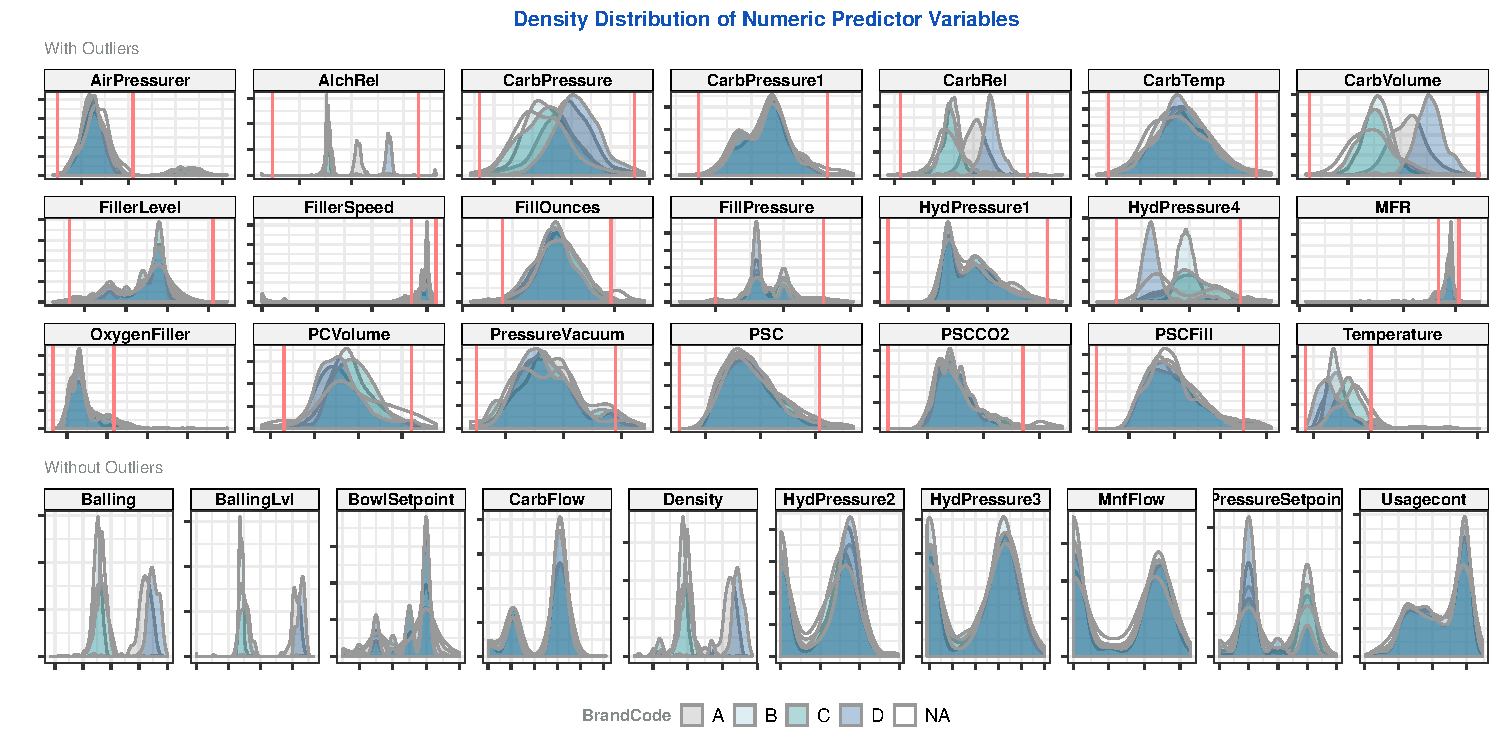
\includegraphics{Group2_Project2_Fall2019_files/figure-latex/unnamed-chunk-4-1.pdf}

\textbf{Cool Plot}

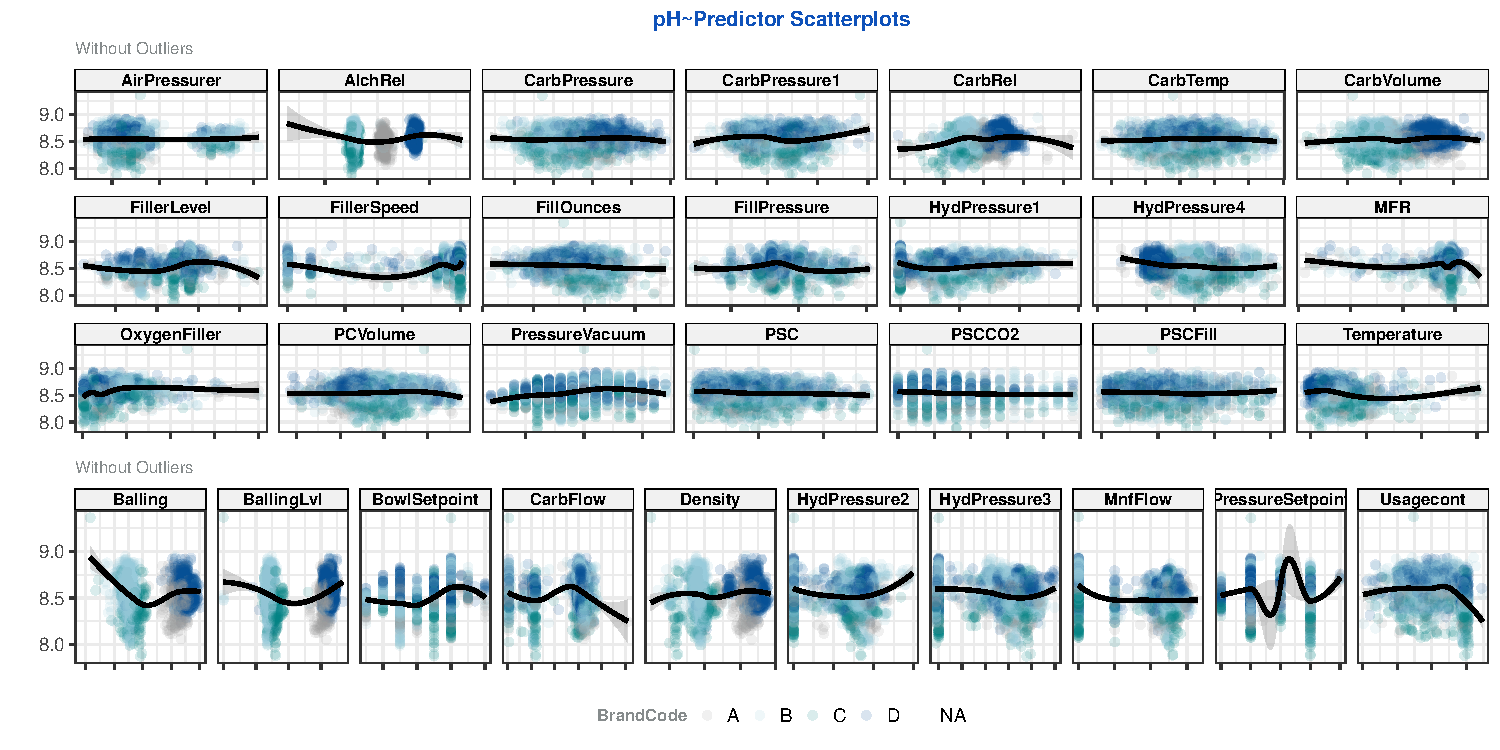
\includegraphics{Group2_Project2_Fall2019_files/figure-latex/unnamed-chunk-5-1.pdf}
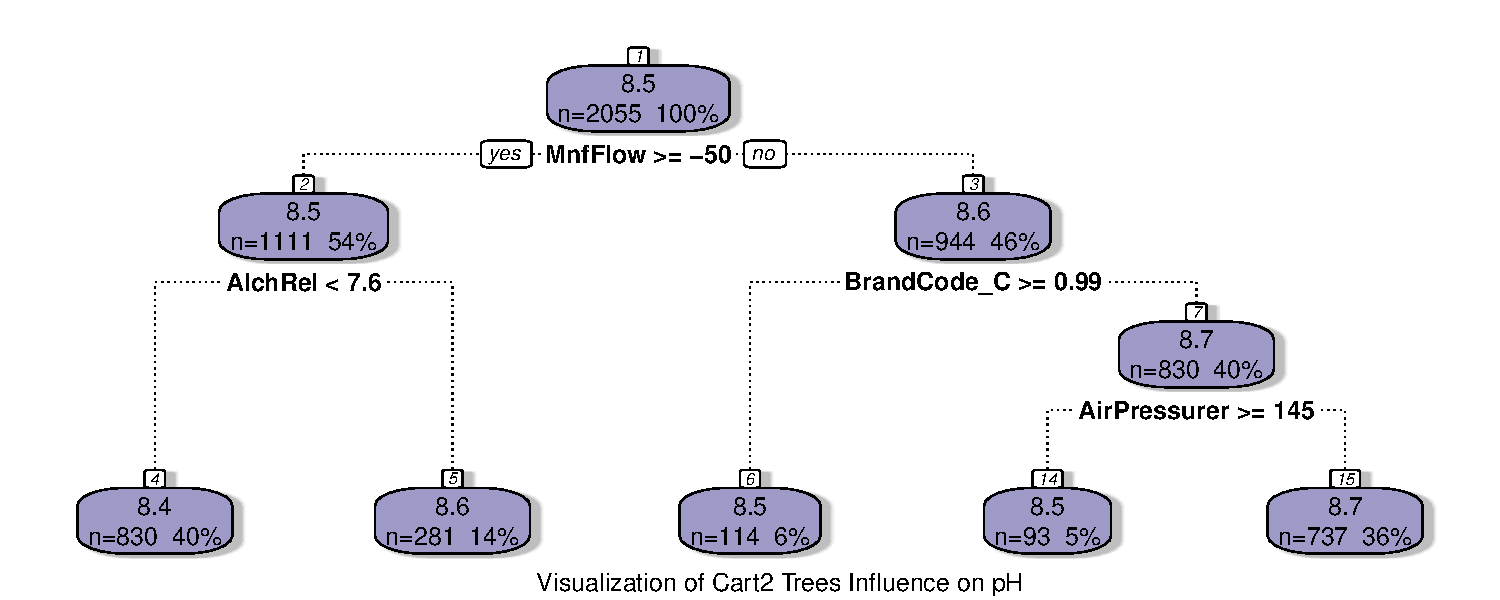
\includegraphics{Group2_Project2_Fall2019_files/figure-latex/unnamed-chunk-5-2.pdf}

\textbf{ALT PLOT}

Do not recomment. Seems much more difficult to customize.

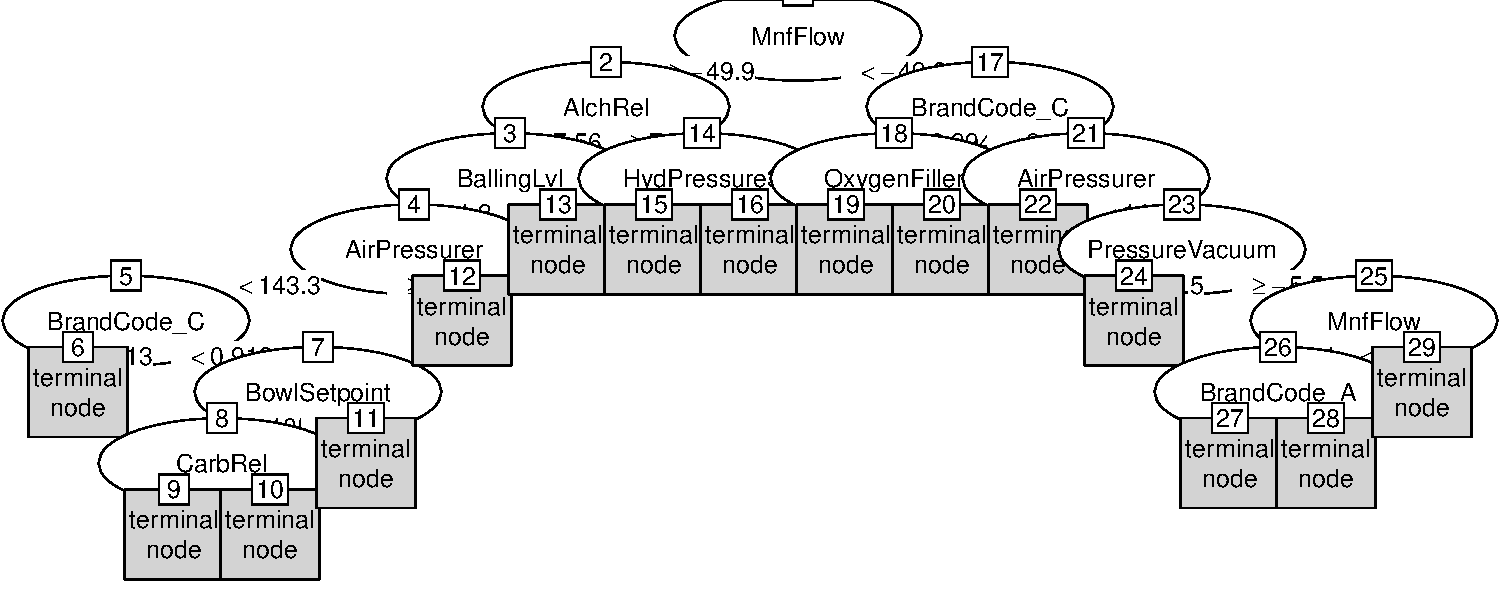
\includegraphics{Group2_Project2_Fall2019_files/figure-latex/unnamed-chunk-6-1.pdf}
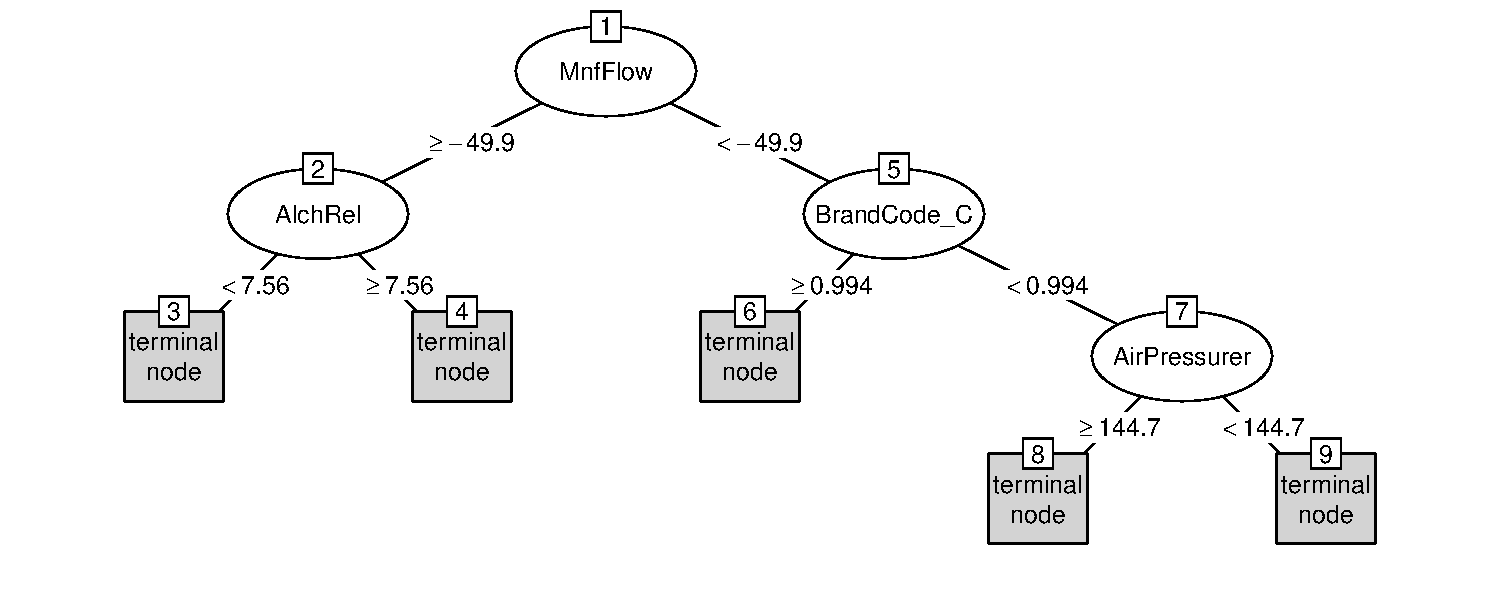
\includegraphics{Group2_Project2_Fall2019_files/figure-latex/unnamed-chunk-6-2.pdf}


\end{document}
